\documentclass[11pt,letterpaper]{article}
\usepackage[utf8]{inputenc}
\usepackage{caption} % for table captions
\usepackage{amsmath} % for multi-line equations and piecewises
\DeclareMathOperator{\sign}{sign}
\usepackage{graphicx}
\usepackage{relsize}
%\usepackage{textcomp}
\usepackage{xspace}
\usepackage{verbatim} % for block comments
%\usepackage{subfig} % for subfigures
\usepackage{enumitem} % for a) b) c) lists
\newcommand{\Cyclus}{\textsc{Cyclus}\xspace}%
\newcommand{\Cycamore}{\textsc{Cycamore}\xspace}%
\usepackage{tabularx}
\usepackage{color}
\usepackage[acronym,toc]{glossaries}
%\newacronym{<++>}{<++>}{<++>}
%\newacronym{<++>}{<++>}{<++>}
\newacronym[longplural={metric tons of heavy metal}]{MTHM}{MTHM}{metric ton of heavy metal}
\newacronym{ABM}{ABM}{agent-based modeling}
\newacronym{AHTR}{AHTR}{Advanced High Temperature Reactor}
\newacronym{ANDRA}{ANDRA}{Agence Nationale pour la gestion des D\'echets RAdioactifs, the French National Agency for Radioactive Waste Management}
\newacronym{ANL}{ANL}{Argonne National Laboratory}
\newacronym{API}{API}{application programming interface}
\newacronym{ARCH}{ARCH}{autoregressive conditional heteroskedastic}
\newacronym{ARE}{ARE}{Aircraft Reactor Experiment}
\newacronym{ARFC}{ARFC}{Advanced Reactors and Fuel Cycles}
\newacronym{ARMA}{ARMA}{autoregressive moving average}
\newacronym{ASME}{ASME}{American Society of Mechanical Engineers}
\newacronym{ATWS}{ATWS}{Anticipated Transient Without Scram}
\newacronym{BDBE}{BDBE}{Beyond Design Basis Event}
\newacronym{BIDS}{BIDS}{Berkeley Institute for Data Science}
\newacronym{CAFCA}{CAFCA}{ Code for Advanced Fuel Cycles Assessment }
\newacronym{CEA}{CEA}{Commissariat \`a l'\'Energie Atomique et aux \'Energies Alternatives}
\newacronym{CI}{CI}{continuous integration}
\newacronym{CNERG}{CNERG}{Computational Nuclear Engineering Research Group}
\newacronym{COSI}{COSI}{Commelini-Sicard}
\newacronym{COTS}{COTS}{commercial, off-the-shelf}
\newacronym{CSNF}{CSNF}{commercial spent nuclear fuel}
\newacronym{CTAH}{CTAHs}{Coiled Tube Air Heaters}
\newacronym{CUBIT}{CUBIT}{CUBIT Geometry and Mesh Generation Toolkit}
\newacronym{DAG}{DAG}{directed acyclic graph}
\newacronym{DANESS}{DANESS}{Dynamic Analysis of Nuclear Energy System Strategies}
\newacronym{DBE}{DBE}{Design Basis Event}
\newacronym{DESAE}{DESAE}{Dynamic Analysis of Nuclear Energy Systems Strategies}
\newacronym{DHS}{DHS}{Department of Homeland Security}
\newacronym{DOE}{DOE}{Department of Energy}
\newacronym{DRACS}{DRACS}{Direct Reactor Auxiliary Cooling System}
\newacronym{DRE}{DRE}{dynamic resource exchange}
\newacronym{DSNF}{DSNF}{DOE spent nuclear fuel}
\newacronym{DYMOND}{DYMOND}{Dynamic Model of Nuclear Development }
\newacronym{EBS}{EBS}{Engineered Barrier System}
\newacronym{EDZ}{EDZ}{Excavation Disturbed Zone}
\newacronym{EPA}{EPA}{Environmental Protection Agency}
\newacronym{EP}{EP}{Engineering Physics}
\newacronym{FCO}{FCO}{Fuel Cycle Options}
\newacronym{FCT}{FCT}{Fuel Cycle Technology}
\newacronym{FEHM}{FEHM}{Finite Element Heat and Mass Transfer}
\newacronym{FEPs}{FEPs}{Features, Events, and Processes}
\newacronym{FHR}{FHR}{Fluoride-Salt-Cooled High-Temperature Reactor}
\newacronym{FLiBe}{FLiBe}{Fluoride-Lithium-Beryllium}
\newacronym{GCAM}{GCAM}{Global Change Assessment Model}
\newacronym{GDSE}{GDSE}{Generic Disposal System Environment}
\newacronym{GDSM}{GDSM}{Generic Disposal System Model}
\newacronym{GENIUSv1}{GENIUSv1}{Global Evaluation of Nuclear Infrastructure Utilization Scenarios, Version 1}
\newacronym{GENIUSv2}{GENIUSv2}{Global Evaluation of Nuclear Infrastructure Utilization Scenarios, Version 2}
\newacronym{GENIUS}{GENIUS}{Global Evaluation of Nuclear Infrastructure Utilization Scenarios}
\newacronym{GPAM}{GPAM}{Generic Performance Assessment Model}
\newacronym{GRSAC}{GRSAC}{Graphite Reactor Severe Accident Code}
\newacronym{GUI}{GUI}{graphical user interface}
\newacronym{HLW}{HLW}{high level waste}
\newacronym{HPC}{HPC}{high-performance computing}
\newacronym{HTC}{HTC}{high-throughput computing}
\newacronym{HTGR}{HTGR}{High Temperature Gas-Cooled Reactor}
\newacronym{IAEA}{IAEA}{International Atomic Energy Agency}
\newacronym{INL}{INL}{Idaho National Laboratory}
\newacronym{JFNK}{JFNK}{Jacobian-Free Newton Krylov}
\newacronym{LANL}{LANL}{Los Alamos National Laboratory}
\newacronym{LBNL}{LBNL}{Lawrence Berkeley National Laboratory}
\newacronym{LCOE}{LCOE}{levelized cost of electricity}
\newacronym{LDRD}{LDRD}{laboratory directed research and development}
\newacronym{LFR}{LFR}{Lead-Cooled Fast Reactor}
\newacronym{LLNL}{LLNL}{Lawrence Livermore National Laboratory}
\newacronym{LMFBR}{LMFBR}{Liquid-Metal-cooled Fast Breeder Reactor}
\newacronym{LOFC}{LOFC}{Loss of Forced Cooling}
\newacronym{LOHS}{LOHS}{Loss of Heat Sink}
\newacronym{LOLA}{LOLA}{Loss of Large Area}
\newacronym{LP}{LP}{linear program}
\newacronym{MARKAL}{MARKAL}{MARKet and ALlocation}
\newacronym{MA}{MA}{minor actinide}
\newacronym{MCNP}{MCNP}{Monte Carlo N-Particle code}
\newacronym{MILP}{MILP}{mixed-integer linear program}
\newacronym{MIT}{MIT}{the Massachusetts Institute of Technology}
\newacronym{MOAB}{MOAB}{Mesh-Oriented datABase}
\newacronym{MOOSE}{MOOSE}{Multiphysics Object-Oriented Simulation Environment}
\newacronym{MOX}{MOX}{mixed oxide}
\newacronym{MSBR}{MSBR}{Molten Salt Breeder Reactor}
\newacronym{MSRE}{MSRE}{Molten Salt Reactor Experiment}
\newacronym{MSR}{MSR}{Molten Salt Reactor}
\newacronym{NAGRA}{NAGRA}{National Cooperative for the Disposal of Radioactive Waste}
\newacronym{NEAMS}{NEAMS}{Nuclear Engineering Advanced Modeling and Simulation}
\newacronym{NEUP}{NEUP}{Nuclear Energy University Programs}
\newacronym{NFCSim}{NFCSim}{Nuclear Fuel Cycle Simulator}
\newacronym{NFC}{NFC}{Nuclear Fuel Cycle}
\newacronym{NGNP}{NGNP}{Next Generation Nuclear Plant}
\newacronym{NNSA}{NNSA}{National Nuclear Security Administration}
\newacronym{NQA1}{NQA-1}{Nuclear Quality Assurance - 1}
\newacronym{NRC}{NRC}{Nuclear Regulatory Commission}
\newacronym{NSF}{NSF}{National Science Foundation}
\newacronym{NSSC}{NSSC}{Nuclear Science and Security Consortium}
\newacronym{NUWASTE}{NUWASTE}{Nuclear Waste Assessment System for Technical Evaluation}
\newacronym{NWTRB}{NWTRB}{Nuclear Waste Technical Review Board}
\newacronym{OCRWM}{OCRWM}{Office of Civilian Radioactive Waste Management}
\newacronym{ORION}{ORION}{ORION}
\newacronym{ORNL}{ORNL}{Oak Ridge National Laboratory}
\newacronym{PARCS}{PARCS}{Purdue Advanced Reactor Core Simulator}
\newacronym{PBAHTR}{PB-AHTR}{Pebble Bed Advanced High Temperature Reactor}
\newacronym{PBFHR}{PB-FHR}{Pebble-Bed Fluoride-Salt-Cooled High-Temperature Reactor}
\newacronym{PEI}{PEI}{Peak Environmental Impact}
\newacronym{PH}{PRONGHORN}{PRONGHORN}
\newacronym{PRKE}{PRKE}{Point Reactor Kinetics Equations}
\newacronym{PSPG}{PSPG}{Pressure-Stabilizing/Petrov-Galerkin}
\newacronym{PWAR}{PWAR}{Pratt and Whitney Aircraft Reactor}
\newacronym{PyNE}{PyNE}{Python toolkit for Nuclear Engineering}
\newacronym{PyRK}{PyRK}{Python for Reactor Kinetics}
\newacronym{QA}{QA}{quality assurance}
\newacronym{RDD}{RD\&D}{Research Development and Demonstration}
\newacronym{RD}{R\&D}{Research and Development}
\newacronym{RELAP}{RELAP}{Reactor Excursion and Leak Analysis Program}
\newacronym{RIA}{RIA}{Reactivity Insertion Accident}
\newacronym{RIF}{RIF}{Region-Institution-Facility}
\newacronym{SFR}{SFR}{Sodium-Cooled Fast Reactor}
\newacronym{SINDAG}{SINDA{\textbackslash}G}{Systems Improved Numerical Differencing Analyzer $\backslash$ Gaski}
\newacronym{SKB}{SKB}{Svensk K\"{a}rnbr\"{a}nslehantering AB}
\newacronym{SNF}{SNF}{spent nuclear fuel}
\newacronym{SNL}{SNL}{Sandia National Laboratory}
\newacronym{STC}{STC}{specific temperature change}
\newacronym{SUPG}{SUPG}{Streamline-Upwind/Petrov-Galerkin}
\newacronym{SWF}{SWF}{Separations and Waste Forms}
\newacronym{SWU}{SWU}{Separative Work Unit}
\newacronym{TRISO}{TRISO}{Tristructural Isotropic}
\newacronym{TSM}{TSM}{Total System Model}
\newacronym{TSPA}{TSPA}{Total System Performance Assessment for the Yucca Mountain License Application}
\newacronym{UFD}{UFD}{Used Fuel Disposition}
\newacronym{UML}{UML}{Unified Modeling Language}
\newacronym{UOX}{UOX}{uranium oxide}
\newacronym{UQ}{UQ}{uncertainty quantification}
\newacronym{US}{US}{United States}
\newacronym{UW}{UW}{University of Wisconsin}
\newacronym{VISION}{VISION}{the Verifiable Fuel Cycle Simulation Model}
\newacronym{VV}{V\&V}{verification and validation}
\newacronym{WIPP}{WIPP}{Waste Isolation Pilot Plant}
\newacronym{YMR}{YMR}{Yucca Mountain Repository Site}

\definecolor{bg}{rgb}{0.95,0.95,0.95}
\newcolumntype{b}{X}
\newcolumntype{f}{>{\hsize=.15\hsize}X}
\newcolumntype{s}{>{\hsize=.5\hsize}X}
\newcolumntype{m}{>{\hsize=.75\hsize}X}
\newcolumntype{r}{>{\hsize=1.1\hsize}X}
\usepackage{titling}
\usepackage[hang,flushmargin]{footmisc}
\renewcommand*\footnoterule{}
\usepackage[newfloat]{minted}
\newenvironment{code}{\captionsetup{type=listing}}{}
\SetupFloatingEnvironment{listing}{name=Code}
\newcolumntype{P}[1]{>{\centering\arraybackslash}p{#1}}

\bibliographystyle{abbrv}
\usepackage{tikz}


\usetikzlibrary{shapes.geometric,arrows}
\tikzstyle{process} = [rectangle, rounded corners, minimum width=1cm, minimum height=1cm,text centered, draw=black, fill=blue!30]
\tikzstyle{arrow} = [thick,->,>=stealth]


\graphicspath{{images/}}
\title{Numerical Experiments for Verifying Demand Driven Deployment Algorithms 
        \\ \vspace{0.5em} Deterministic-Optimizing Algorithm}
\author{Jin Whan Bae, Gwendolyn Chee, Kathryn Huff}


\begin{document}
	\maketitle
	\hrule

\section{Introduction}
For many fuel cycle simulations, it is currently up to the user to define
a deploy scheme, or facility parameters, to make sure that there's no gap
in the supply chain. Or, the same goal is achieved by setting the
\texttt{facility} capacity to infinity, which does not reflect real-world
conditions. 

The Demand-Driven Cycamore Archetype project (NEUP-FY16-10512) aims to develop \Cycamore demand-driven deployment capabilities.
The developed algorithm, in the form of \Cyclus \texttt{Institution}
agent, deploys \texttt{Facilities} to meet the front-end and back-end demands of the 
fuel cycle.

This report describes numerical experiments for the deterministic
-optimizing algorithm, namely \gls{ARMA} and \gls{ARCH}.

These prediction models are being developed by the University of South Carolina. The numerical experiments will be designed for both
 the once through nuclear fuel 
cycle and advanced fuel cycles. 

\section{Method}
This report lists necessary capabilities of the new \Cyclus \texttt{institute}
for demand-driven deployment of fuel cycle facilities. 
Then the report lists tests to check correct implementation of the capabilities,
with a sample fuel cycle with well-defined facility parameters.


\section{Configuration}
The user defines a demand equation of a commodity (e.g. power, spent fuel, plutonium etc.)
and a supply chain that results in the creation of the demanded commodity.
For example, a user would define a power demand equation, and list
the facilities that lead up to power production, as such:

\begin{minted}{xml}
<!-- Definition of demand commodity and demand equation -->
<demand_commodity> POWER </demand_commodity>
<piecewise_function>
	<piece>
		<start>0</start>
		<function>
			<type>linear</type>
			<params> 1 2 </params>
		</function>
	</piece>
</piecewise_function>

<!-- Definition of supply chain leading to power production -->
<supply_chain>
	<val> source </val>
	<val> enrichment </val>
	<val> reactor </val>
</supply_chain>
\end{minted}



\section{Algorithm Flow}

The algorithm is an \texttt{Institution}, which is a \Cyclus agent type
that deploys and decommissions facilities.

Upon entering, the \Cyclus \texttt{institute} accesses the parameters for each
facility in the chain to extract the supply and demand parameters (capacity, throughput).
The algorithm then creates a matrix of commodity demand quantities for every
facility of the supply chain. It does so by first creating a vector
of the final demand (e.g. power) and back-calculating the demand for other
commodities in order to meet power production demand.
The matrix has a size of \texttt{(Timestep X Length of Chain)}.
The demand quantity matrix is then calculated into a deployment matrix that
lists the number of facilities to be deployed at a given timestep.


\subsection{Specifics}


\subsection{Time Step Execution in \Cyclus}
As a reference, the time step execution for \Cyclus is illustrated in figure \ref{diag:time}.

At \texttt{Tock}, the algorithm calculates the demand and supply for the next timestep, and calculates
the difference. If the difference is bigger than the capacity of one facility, it
schedules to deploy a new facility, or a decommissioning of an existing facility.
The decommissioning takes place in the \texttt{Decommission} phase of \Cyclus, and
the construction takes place in the \texttt{Build} phase of \Cyclus. Thus, all the
adjustment of facilities occur prior to the next \gls{DRE}.


\begin{figure}[H]
\centering
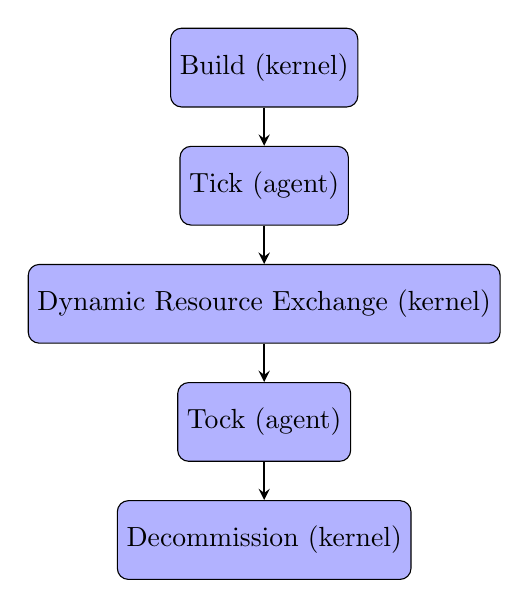
\begin{tikzpicture}[node distance=1.5cm]
\node (Build) [process] {Build (kernel)};
\node (Tick) [process, below of=Build] {Tick (agent)};
\node (DRE) [process, below of=Tick]{Dynamic Resource Exchange (kernel) };
\node (Tock) [process, below of=DRE]{Tock (agent)};
\node (Decom) [process, below of=Tock] {Decommission (kernel)};

\draw [arrow] (Build) -- (Tick); 
\draw [arrow] (Tick) -- (DRE);
\draw [arrow] (DRE) -- (Tock);
\draw [arrow] (Tock) -- (Decom);
\end{tikzpicture}
\caption{Each timestep in \Cyclus follows the five steps in order. Processes labeled
         kernel are executed by the \Cyclus framework, whereas processes labeled agent
         are executed by individual agents. What happens in the `Tick' and `Tock' is
         thus unique to each archetype.}
\label{diag:time}
\end{figure}


\section{Simulation parameter for Test Scenarios}
Simple parameters are given to fuel cycle facilities for the numerical testing of 
the algorithm.  Only \texttt{source} and \texttt{reactor} facilities are used in the test scenarios. 

Table \ref{tab:testscenario} provides basic parameters for each test scenario. Table \ref{tab:reactor} provides the parameters for the \texttt{source}, \texttt{reactors} and \texttt{sink} in the test scenarios.

\begin{table}[H]
	\centering
	\caption {Basic Test Parameters}
	\label{tab:testscenario}
	\begin{tabular}{|l|l|l|}
		\hline
		\textbf{Test Scenario Parameters} & \textbf{Value} & \textbf{Units} \\
		\hline
		Duration & 15 & timesteps \\
		Timestep & 1 & month \\
		Start Month & 1 & month \\
		Start Year & 2000 & year \\
		\hline
	\end{tabular}
\end{table}

\begin{table}[H]
	\centering
    \caption {Source, Reactor and Sink Parameters}
	\label{tab:reactor}
	\begin{tabular}{|l|l|l|}
\hline
\textbf{Source Parameters} & \textbf{Value} & \textbf{Units} \\
\hline
Throughput & 1 & kg \\
Output Commodity & fuel & kg\\
\hline
\textbf{Reactor Parameters} & \textbf{Value} & \textbf{Units} \\
\hline
Cycle Time & 1 & timesteps \\
Refuel Time & 0 & timesteps \\
Lifetime & 1 & timesteps \\
Power Capacity & 1& MWe \\
Assembly Size & 1 & kg \\
\# assemblies per core & 1 & \\
\# assemblies per batch & 1 & \\
Input Commodity & fuel & kg\\
Output Commodity & power & MW\\
\hline
\textbf{Sink Parameters} & \textbf{Value} & \textbf{Units} \\
Throughput & 1 & kg \\
Input Commodity & spent uox & kg\\
\hline
	\end{tabular}
\end{table}

\pagebreak

\section{Numerical Tests for the Non-optimizing prediction method}
The non-optimizing prediction method is tested by comparing its output for various scenarios against their analytical solutions . In this section, the tests that must be met is described based on the parameters defined in table \ref{tab:testscenario} and \ref{tab:reactor} and analytical solution of a defined simple scenario. Unit test examples are included in Appendix B.

The tests are split into test A types and test B types. Test A refers to the test scenarios where facilities are expected to be deployed. Test B refers to the test scenarios where facilities are expected to be decommissioned. 

The prediction algorithm for the non-optimizing method has three user-defined input parameters. The aim of the various test scenarios are to check if the non-optimizing method archetype will deploy or decommission facilities correctly when there is a variation in the combination of the three input parameters.  The input parameters are: 
\begin{enumerate}
	\item Initial demand value  
	\item Number of initial facilities (initial supply)
	\item Growth rate of initial demand
\end{enumerate}

The growth in demand is governed by the Equation \ref{eq:growth}. 

\begin{align}
\label{eq:growth}
D_f(timestep) &= D_i(1+g)^{(\frac{timestep}{12})}
\end{align}
Where $D_f$ is demand of resource at specific time step, $D_i$ is initial demand and g is growth rate. 

\texttt{Source} and \texttt{reactor} facilities are used in the test scenarios. Test scenarios A1 to A4 and B1 to B2 only have a \texttt{source} facility and test scenarios A5 to A7 have both \texttt{source} and \texttt{reactor} facilities. For each test scenario, there is one table that states the test scenario's input parameters and another table that states the exact analytical solution. The analytical solution table does not include deployment of the initial facility that is stated in the first table.

Additionally, we created base tests for each A-type test scenario that passes when the supply meets the demand within a given facility number tolerance. In other words, when the supply exceeds the demand by the specified tolerance quantity, the test still passes. For this report, the tolerance is set to one facility. For example in test A-1, the expected total number facilities deployed is 1, and since the facility over-prediction tolerance is 1, the acceptable range of total number of facilities $(x)$ deployed in the entire test scenario is $1<x<2$. If the total number of facilities deployed is within this range, the base case test will pass.  

\subsection{Test A-1}
In test A-1, only a \texttt{source} facility is present in the test scenario. Table \ref{tab:testa1} shows the input parameters of the source facility in the test scenario. Table \ref{tab:testa1ana} shows the expected analytical solution based on the test scenario. Table \ref{tab:testa1base} shows the accepted range of total number of facilities deployed over the test scenario which will pass the base test, which factors in the facility over-prediction tolerance of 1. 
\begin{table}[H]
	\centering
	\caption{Test A-1 Scenario Input Parameters }
	\label{tab:testa1}
	\begin{tabular}{|l|l|l|}
		\hline
		\textbf{Source Parameter} & \textbf{Value} & \textbf{Units} \\
		\hline
		Initial demand & 1 & kg \\
		Initial facilities & 0 & \#\\
		Growth Rate & 0 & \\
\hline
	\end{tabular}
\end{table}

\begin{table}[H]
	\centering
	\caption{Test A-1 Analytical Solution}
	\label{tab:testa1ana}
	\begin{tabular}{|l|l|}
		\hline
		\textbf{Time Step} & \textbf{\shortstack{No. of Source \\Facilities Deployed}}\\
		\hline
		1 & 1\\
		2 to 15& 0 \\
		\hline
	\end{tabular}
\end{table}

\begin{table}[H]
	\centering
	\caption{Test A-1 Base Test Acceptance}
	\label{tab:testa1base}
	\begin{tabular}{|P{6.5cm}|}
		\hline
		\textbf{\shortstack{Acceptable total No. of Source \\Facilities Deployed + tolerance}}\\
		\hline
		1 $<$ x $<$ 2 \\
		\hline
	\end{tabular}
\end{table}

\subsection{Test A-2}
In test A-2, only a \texttt{source} facility is present in the test scenario. Table \ref{tab:testa2} shows the input parameters of the source facility in the test scenario. Table \ref{tab:testa2ana} shows the expected analytical solution based on the test scenario.Table \ref{tab:testa2base} shows the accepted range of total number of facilities deployed over the test scenario which will pass the base test, which factors in the facility over-prediction tolerance of 1. 

\begin{table}[H]
	\centering
	\caption{Test A-2 Scenario Input Parameters }
	\label{tab:testa2}
	\begin{tabular}{|l|l|l|}
		\hline
		\textbf{Source Parameter} & \textbf{Value} & \textbf{Units} \\
		\hline
		Initial demand & 2 & kg \\
		Initial facilities & 1 & \#\\
		Growth Rate & 0 & \\
		\hline
	\end{tabular}
\end{table}

\begin{table}[H]
	\centering
	\caption{Test A-2 Analytical Solution}
	\label{tab:testa2ana}
	\begin{tabular}{|l|l|}
		\hline
		\textbf{Time Step} & \textbf{\shortstack{No. of Source \\Facilities Deployed}}\\
		\hline
		1 & 1\\
		2 to 15& 0 \\
		\hline
	\end{tabular}
\end{table}

\begin{table}[H]
	\centering
	\caption{Test A-2 Base Test Acceptance}
	\label{tab:testa2base}
	\begin{tabular}{|P{6.5cm}|}
		\hline
		\textbf{\shortstack{Acceptable total No. of Source \\Facilities Deployed + tolerance}}\\
		\hline
		2 $<$ x $<$ 3 \\
		\hline
	\end{tabular}
\end{table}

\subsection{Test A-3}
In test A-3, only a \texttt{source} facility is present in the test scenario. Table \ref{tab:testa3} shows the input parameters of the source facility in the test scenario. Table \ref{tab:testa3ana} shows the expected analytical solution based on the test scenario. Table \ref{tab:testa3base} shows the accepted range of total number of facilities deployed over the test scenario which will pass the base test, which factors in the facility over-prediction tolerance of 1. 

\begin{table}[H]
	\centering
	\caption{Test A-3 Scenario Input Parameters}
	\label{tab:testa3}
	\begin{tabular}{|l|l|l|}
		\hline
		\textbf{Source Parameter} & \textbf{Value} & \textbf{Units} \\
		\hline
		Initial demand & 1 & kg \\
		Initial facilities & 0 & \#\\
		Growth Rate & 1 &  \\
		\hline
	\end{tabular}
\end{table}

\begin{table}[H]
	\centering
	\caption{Test A-3 Analytical Solution}
	\label{tab:testa3ana}
	\begin{tabular}{|l|l|}
		\hline
		\textbf{Time Step} & \textbf{\shortstack{No. of Source \\Facilities Deployed}}\\
		\hline
		1 & 2\\
		2 to 12 & 0 \\
		13 & 1 \\
		14 to 15 & 0 \\
		\hline
	\end{tabular}
\end{table}

\begin{table}[H]
	\centering
	\caption{Test A-3 Base Test Acceptance}
	\label{tab:testa3base}
	\begin{tabular}{|P{6.5cm}|}
		\hline
		\textbf{\shortstack{Acceptable total No. of Source \\Facilities Deployed + tolerance}}\\
		\hline
		3 $<$ x $<$ 4 \\
		\hline
	\end{tabular}
\end{table}

\subsection{Test A-4}
In test A-4, only a \texttt{source} facility is present in the test scenario. Table \ref{tab:testa4} shows the input parameters of the source facility in the test scenario. Table \ref{tab:testa4ana} shows the expected analytical solution based on the test scenario. Table \ref{tab:testa4base} shows the accepted range of total number of facilities deployed over the test scenario which will pass the base test, which factors in the facility over-prediction tolerance of 1. 

\begin{table}[H]
	\centering
	\caption{Test A-4 Scenario Input Parameters }
	\label{tab:testa4}
	\begin{tabular}{|l|l|l|}
		\hline
		\textbf{Source Parameter} & \textbf{Value} & \textbf{Units} \\
		\hline
		Initial demand & 1 & kg \\
		Initial facilities & 1 & \#\\
		Growth Rate & 1 &  \\
		\hline
	\end{tabular}
\end{table}

\begin{table}[H]
	\centering
	\caption{Test A-4 Analytical Solution}
	\label{tab:testa4ana}
	\begin{tabular}{|l|l|}
		\hline
		\textbf{Time Step} & \textbf{\shortstack{No. of Source \\Facilities Deployed}}\\
		\hline
		1 & 1\\
		2 to 12 & 0 \\
		13 & 1 \\
		14 to 15 & 0 \\
		\hline
	\end{tabular}
\end{table}

\begin{table}[H]
	\centering
	\caption{Test A-4 Base Test Acceptance}
	\label{tab:testa4base}
	\begin{tabular}{|P{6.5cm}|}
		\hline
		\textbf{\shortstack{Acceptable total No. of Source \\Facilities Deployed + tolerance}}\\
		\hline
		3 $<$ x $<$ 4 \\
		\hline
	\end{tabular}
\end{table}

\subsection{Test A-5}
In test A-5, both a \texttt{source} and \texttt{reactor} facility is present in the test scenario. Table \ref{tab:testa5} shows the input parameters of the source facility in the test scenario. Table \ref{tab:testa5ana} shows the expected analytical solution based on the test scenario. Table \ref{tab:testa5base} shows the accepted range of total number of facilities deployed over the test scenario which will pass the base test, which factors in the facility over-prediction tolerance of 1. 

\begin{table}[H]
	\centering
	\caption{Test A-5 Scenario Input Parameters}
	\label{tab:testa5}
	\begin{tabular}{|l|l|l|}
		\hline
		\textbf{Source Parameter} & \textbf{Value} & \textbf{Units} \\
		\hline
		Initial demand & 1 & kg \\
		Initial facilities & 0 & \#\\
		Growth Rate & 0 &  \\
		\hline
		\textbf{Reactor Parameter} & \textbf{Value} & \textbf{Units} \\
		\hline
		Initial demand & 1 & MW \\
		Initial facilities & 0 & \#\\
		Growth Rate & 0 &  \\
		\hline
	\end{tabular}
\end{table}

\begin{table}[H]
	\centering
	\caption{Test A-5 Analytical Solution}
	\label{tab:testa5ana}
	\begin{tabular}{|l|l|l|}
		\hline
		\textbf{Time Step} & \textbf{\shortstack{No. of Source \\Facilities Deployed}} & \textbf{\shortstack{No. of Reactor \\Facilities Deployed}}\\
		\hline
		1 & 1 & 1\\
		2 to 15 & 0 & 0\\
		\hline
	\end{tabular}
\end{table}

\begin{table}[H]
	\centering
	\caption{Test A-5 Base Test Acceptance}
	\label{tab:testa5base}
	\begin{tabular}{|P{6.5cm}|P{6.5cm}|}
		\hline
		\textbf{\shortstack{Acceptable total No. of Source \\Facilities Deployed + tolerance}} &\textbf{\shortstack{Acceptable total No. of Reactor \\Facilities Deployed + tolerance}}\\
		\hline
		1 $<$ x $<$ 2 & 1 $<$ x $<$ 2\\
		\hline
	\end{tabular}
\end{table}

\subsection{Test A-6}
In test A-6, both a \texttt{source} and \texttt{reactor} facility is present in the test scenario. Table \ref{tab:testa6} shows the input parameters of the source facility in the test scenario. Table \ref{tab:testa6ana} shows the expected analytical solution based on the test scenario. Table \ref{tab:testa6base} shows the accepted range of total number of facilities deployed over the test scenario which will pass the base test, which factors in the facility over-prediction tolerance of 1. 

\begin{table}[H]
	\centering
	\caption{Test A-6 Scenario Input Parameters }
	\label{tab:testa6}
	\begin{tabular}{|l|l|l|}
		\hline
		\textbf{Source Parameter} & \textbf{Value} & \textbf{Units} \\
		\hline
		Initial demand & 1 & kg \\
		Initial facilities & 1 & \#\\
		Growth Rate & 0 &  \\
		\hline
		\textbf{Reactor Parameter} & \textbf{Value} & \textbf{Units} \\
		\hline
		Initial demand & 1 & MW \\
		Initial facilities & 1 & \#\\
		Growth Rate & 0 &  \\
		\hline
	\end{tabular}
\end{table}

\begin{table}[H]
	\centering
	\caption{Test A-6 Analytical Solution}
	\label{tab:testa6ana}
	\begin{tabular}{|l|l|l|}
		\hline
		\textbf{Time Step} & \textbf{\shortstack{No. of Source \\Facilities Deployed}} & \textbf{\shortstack{No. of Reactor \\Facilities Deployed}}\\
		\hline
		1 & 1 & 1\\
		2 to 15 & 0 & 0\\
		\hline
	\end{tabular}
\end{table}

\begin{table}[H]
	\centering
	\caption{Test A-6 Base Test Acceptance}
	\label{tab:testa6base}
	\begin{tabular}{|P{6.5cm}|P{6.5cm}|}
		\hline
		\textbf{\shortstack{Acceptable total No. of Source \\Facilities Deployed + tolerance}} &\textbf{\shortstack{Acceptable total No. of Reactor \\Facilities Deployed + tolerance}}\\
		\hline
		1 $<$ x $<$ 2 & 1 $<$ x $<$ 2\\
		\hline
	\end{tabular}
\end{table}

\subsection{Test A-7}
In test A-7, both a \texttt{source} and \texttt{reactor} facility is present in the test scenario. Table \ref{tab:testa7} shows the input parameters of the source facility in the test scenario. Table \ref{tab:testa7ana} shows the expected analytical solution based on the test scenario. Table \ref{tab:testa7base} shows the accepted range of total number of facilities deployed over the test scenario which will pass the base test, which factors in the facility over-prediction tolerance of 1. 


\begin{table}[H]
	\centering
	\caption{Test A-7 Scenario Input Parameters }
	\label{tab:testa7}
	\begin{tabular}{|l|l|l|}
		\hline
		\textbf{Source Parameter} & \textbf{Value} & \textbf{Units} \\
		\hline
		Initial demand & 1 & kg \\
		Initial facilities & 0 & \#\\
		Growth Rate & 1 &  \\
		\hline
		\textbf{Reactor Parameter} & \textbf{Value} & \textbf{Units} \\
		\hline
		Initial demand & 1 & MW \\
		Initial facilities & 0 & \#\\
		Growth Rate & 1 &  \\
		\hline
	\end{tabular}
\end{table}

\begin{table}[H]
	\centering
	\caption{Test A-7 Analytical Solution}
	\label{tab:testa7ana}
	\begin{tabular}{|l|l|l|}
		\hline
		\textbf{Time Step} & \textbf{\shortstack{No. of Source \\Facilities Deployed}} & \textbf{\shortstack{No. of Reactor \\Facilities Deployed}}\\
		\hline
		1 & 2 & 2\\
		2 to 12 & 0 & 0\\
		13 & 1 & 1\\
		14 to 15 & 0 & 0\\
		\hline
	\end{tabular}
\end{table}

\begin{table}[H]
	\centering
	\caption{Test A-7 Base Test Acceptance}
	\label{tab:testa6base}
	\begin{tabular}{|P{6.5cm}|P{6.5cm}|}
		\hline
		\textbf{\shortstack{Acceptable total No. of Source \\Facilities Deployed + tolerance}} &\textbf{\shortstack{Acceptable total No. of Reactor \\Facilities Deployed + tolerance}}\\
		\hline
		3 $<$ x $<$ 4 & 3 $<$ x $<$ 4\\
		\hline
	\end{tabular}
\end{table}

\subsection{Test B-1}
In test B-1, only a \texttt{source} facility is present in the test scenario. Table \ref{tab:testb1} shows the input parameters of the source facility in the test scenario. Table \ref{tab:testb1ana} shows the expected analytical solution based on the test scenario. 

\begin{table}[H]
	\centering
	\caption{Test B-1 Scenario Input Parameters }
	\label{tab:testb1}
	\begin{tabular}{|l|l|l|}
		\hline
		\textbf{Source Parameter} & \textbf{Value} & \textbf{Units} \\
		\hline
		Initial demand & 0 & kg \\
		Initial facilities & 1 & \#\\
		Growth Rate & 0 &  \\
		\hline
	\end{tabular}
\end{table}

\begin{table}[H]
	\centering
	\caption{Test B-1 Analytical Solution}
	\label{tab:testb1ana}
	\begin{tabular}{|l|l|l|}
		\hline
		\textbf{Time Step} & \textbf{\shortstack{No. of Source \\Facilities Deployed}}& \textbf{\shortstack{No. of Source \\Facilities Decomissioned}}\\
		\hline
		1 & 1 & 0\\
		2 & 0 & 1\\
		3 to 15 & 0 & 0\\
		\hline
	\end{tabular}
\end{table}

\subsection{Test B-2}
In test B-2, only a \texttt{source} facility is present in the test scenario. Table \ref{tab:testb2} shows the input parameters of the source facility in the test scenario. Table \ref{tab:testb2ana} shows the expected analytical solution based on the test scenario.

\begin{table}[H]
	\centering
	\caption{Test B-2 Scenario Input Parameters }
	\label{tab:testb2}
	\begin{tabular}{|l|l|l|}
		\hline
		\textbf{Source Parameter} & \textbf{Value} & \textbf{Units} \\
		\hline
		Initial demand & 1 & kg \\
		Initial facilities & 1 & \#\\
		Growth Rate & -1 &  \\
		\hline
	\end{tabular}
\end{table}

\begin{table}[H]
	\centering
	\caption{Test B-2 Analytical Solution}
	\label{tab:testb2ana}
	\begin{tabular}{|l|l|l|}
		\hline
		\textbf{Time Step} & \textbf{\shortstack{No. of Source \\Facilities Deployed}}& \textbf{\shortstack{No. of Source \\Facilities Decomissioned}}\\
		\hline
		1 to 12 & 1 & 0\\
		13 & 0 & 1\\
		14 to 15 & 0 & 0\\
		\hline
	\end{tabular}
\end{table}

\section{Numerical Test Results}
It was found that none of the exact tests and base case tests passed. 
The failures are attributed to three reasons:

\begin{enumerate}
	\item There is a test failure when there is no initial facility present. An initial condition must be given for the algorithm to understand the capacity of the facility it deploys.
	\item There is a test failure when there is growth in the demandhe algorithm failed to deploy facilities to meet the increase in demand.
	\item There is a test failure when facilities are expected to be decommissioned. There is yet to be an implementation on decommissioning behavior.
\end{enumerate}

Despite failures in these situations, the non-optimizing method proved to have commissioning capabilities
to meet demand. Because of the limitation in the algorithm, it is hard to predict demand with precision
in such a short time. However, the same numerical experiments can be applied to the deterministic
optimizing algorithm, which holds more promise. The goal is that the deterministic optimization method
will be able to overcome the issues faced by the non-optimizing method with reference to the
requirement of an initial condition, growth in demand. Also, the capability to decommission facilities
upon oversupply will be added.

Appendix C reflects the numerical experiment solution output by the non-optimizing prediction algorithm for each test scenario defined in section 6. 

\pagebreak

\section{References}
\bibliography{bibliography}

\pagebreak

\section*{Appendix A - parameter configuration}
Appendix A shows the json file that contains the simulation parameters that are common between all the test scenarios discussed in Section 6.  

\begin{minted}{json}
template = {
"simulation": {
"archetypes": {
"spec": [
{"lib": "agents", "name": "NullRegion"}, 
{"lib": "cycamore", "name": "Source"}, 
{"lib": "cycamore", "name": "Reactor"},
{"lib": "cycamore", "name": "Sink"},
{"lib": "d3ploy.no_inst", "name": "NOInst"}
]
}, 
"control": {"duration": "15", "startmonth": "1", "startyear": "2000"}, 
"recipe": [
{
"basis": "mass", 
"name": "fresh_uox", 
"nuclide": [{"comp": "0.711", "id": "U235"}, {"comp": "99.289", "id": "U238"}]
}, 
{
"basis": "mass", 
"name": "spent_uox", 
"nuclide": [{"comp": "50", "id": "Kr85"}, {"comp": "50", "id": "Cs137"}]
}
], 
"facility": [{
"config": {"Source": {"outcommod": "fuel",
"outrecipe": "fresh_uox",
"throughput": "1",
"source_record_supply": "fuel"}}, 
"name": "source"
},
{
"config": {"Sink": {"in_commods": {"val":"spent_uox"},
"max_inv_size": 1,
"sink_record_demand": "fuel_cap"}}, 
"name": "sink"
},
{
"config": {
"Reactor":{
"assem_size":"1",
"cycle_time": "1", 
"fuel_incommods": {"val": "fuel"}, 
"fuel_inrecipes": {"val": "fresh_uox"}, 
"fuel_outcommods": {"val": "spent_uox"}, 
"fuel_outrecipes": {"val": "spent_uox"}, 
"n_assem_batch": "1", 
"n_assem_core": "1", 
"power_cap": "1", 
"refuel_time": "0",
"reactor_fuel_demand": "fuel_reactor"
}
},
"name": "reactor"
}]}}
\end{minted}

\pagebreak
\section*{Appendix B - Sample Test Code }
\subsection*{Sample test code for test A-1}
Appendix B shows the python file that contains the a segment of the simulation parameters that are unique to test A-1 and the code for test A-1. 
\begin{minted}{python}
# Test A_1
INIT_DEMAND = copy.deepcopy(TEMPLATE)
INIT_DEMAND["simulation"].update({"region": {
"config": {"NullRegion": "\n      "},
"institution": {
"config": {
"NOInst": {
"calc_method": "arma",
"demand_commod": "POWER",
"demand_std_dev": "0.0",
"growth_rate": "0.0",
"initial_demand": "1",
"prototypes": {"val": "source"},
"steps": "1",
"supply_commod": "fuel"
}
},
"name": "source_inst"
},
"name": "SingleRegion"
}})

@pytest.mark.base
def test_a1_init_demand():
# tests if NOInst deploys a source
# given initial demand and no initial facilities
output_file = 'init_file.sqlite'
input_file = output_file.replace('.sqlite', '.json')
with open(input_file, 'w') as f:
json.dump(INIT_DEMAND, f)
s = subprocess.check_output(['cyclus', '-o', output_file, input_file],
universal_newlines=True, env=ENV)
# check if ran successfully
assert("Cyclus run successful!" in s)

# getting the sqlite file
cur = get_cursor(output_file)

# check base solution
source_base = cur.execute(query).fetchone()
assert(1 <= source_base[0] <= (1 + tol))

@pytest.mark.exact
def test_a1_init_demand_exact():
output_file = 'init_file.sqlite'
cur = get_cursor(output_file)
# check exact solution
source_exact = cur.execute(query + " AND EnterTime = 1").fetchone()
assert(source_exact[0] == 1)
\end{minted}

\pagebreak

\section*{Appendix C - Numerical Experiment Solution for test scenarios}
\subsection*{Test A-1}
\begin{table}[H]
	\centering
	\caption{Test A-1 Numerical Experiment Solution}
	\label{tab:testa1num}
	\begin{tabular}{|l|l|}
		\hline
		\textbf{Time Step} & \textbf{\shortstack{No. of Source \\Facilities Deployed}}\\
		\hline
		1 to 15& 0\\
		\hline
	\end{tabular}
\end{table}

\subsection*{Test A-2}
\begin{table}[H]
	\centering
	\caption{Test A-2 Numerical Experiment Solution}
	\label{tab:testa2num}
	\begin{tabular}{|l|l|}
		\hline
		\textbf{Time Step} & \textbf{\shortstack{No. of Source \\Facilities Deployed}}\\
		\hline
		1 & 0\\
		2 & 1\\
		3 & 1\\
		4 & 1 \\
		5 & 0 \\
		6 & 1 \\
		7 to 15 & 0 \\
		\hline
	\end{tabular}
\end{table}

\subsection*{Test A-3}
\begin{table}[H]
	\centering
	\caption{Test A-3 Numerical Experiment Solution}
	\label{tab:testa3num}
	\begin{tabular}{|l|l|}
		\hline
		\textbf{Time Step} & \textbf{\shortstack{No. of Source \\Facilities Deployed}}\\
		\hline
		1 to 15& 0\\
		\hline
	\end{tabular}
\end{table}

\subsection*{Test A-4}
\begin{table}[H]
	\centering
	\caption{Test A-4 Numerical Experiment Solution}
	\label{tab:testa4num}
	\begin{tabular}{|l|l|}
		\hline
		\textbf{Time Step} & \textbf{\shortstack{No. of Source \\Facilities Deployed}}\\
		\hline
		1 to 15& 0\\
		\hline
	\end{tabular}
\end{table}

\subsection*{Test A-5}
\begin{table}[H]
	\centering
	\caption{Test A-5 Numerical Experiment Solution}
	\label{tab:testa5num}
	\begin{tabular}{|l|l|l|}
		\hline
		\textbf{Time Step} & \textbf{\shortstack{No. of Source \\Facilities Deployed}} & \textbf{\shortstack{No. of Reactor \\Facilities Deployed}}\\
		\hline
		1 to 15 & 0 & 0\\
		\hline
	\end{tabular}
\end{table}

\subsection*{Test A-6}
\begin{table}[H]
	\centering
	\caption{Test A-6 Numerical Experiment Solution}
	\label{tab:testa6num}
	\begin{tabular}{|l|l|l|}
		\hline
		\textbf{Time Step} & \textbf{\shortstack{No. of Source \\Facilities Deployed}} & \textbf{\shortstack{No. of Reactor \\Facilities Deployed}}\\
		\hline
		1 & 0 & 0\\
		2 & 1 & 0\\
		3 & 1 & 0\\
		4 & 1 & 0\\
		5 & 0 & 0\\
		6 & 1 & 0\\
		7 to 15 & 0 & 0\\
		\hline
	\end{tabular}
\end{table}

\subsection*{Test A-7}
\begin{table}[H]
	\centering
	\caption{Test A-7 Numerical Experiment Solution}
	\label{tab:testa7num}
	\begin{tabular}{|l|l|l|}
		\hline
		\textbf{Time Step} & \textbf{\shortstack{No. of Source \\Facilities Deployed}} & \textbf{\shortstack{No. of Reactor \\Facilities Deployed}}\\
		\hline
		1 to 15 & 0 & 0\\
		\hline
	\end{tabular}
\end{table}

\subsection*{Test B-1}
\begin{table}[H]
	\centering
	\caption{Test B-1 Numerical Experiment Solution}
	\label{tab:testb1num}
	\begin{tabular}{|l|l|l|}
		\hline
		\textbf{Time Step} & \textbf{\shortstack{No. of Source \\Facilities Deployed}}& \textbf{\shortstack{No. of Source \\Facilities Decomissioned}}\\
		\hline
		1 to 15 & 0 & 0\\
		\hline
	\end{tabular}
\end{table}

\subsection*{Test B-2}
\begin{table}[H]
	\centering
	\caption{Test B-2 Numerical Experiment Solution}
	\label{tab:testb2num}
	\begin{tabular}{|l|l|l|}
		\hline
		\textbf{Time Step} & \textbf{\shortstack{No. of Source \\Facilities Deployed}}& \textbf{\shortstack{No. of Source \\Facilities Decomissioned}}\\
		\hline
		1 to 15 & 0 & 0\\
		\hline
	\end{tabular}
\end{table}

\end{document}



